% ============================================================
\section{Intelligenza Artificiale nelle IT Operations}
% ============================================================

% ------------------------------------------------------------
\subsection{Il Contesto Tecnologico e la Necessità dell'AI}
% ------------------------------------------------------------

L'attuale panorama tecnologico è caratterizzato da una crescita
esponenziale nella generazione dei dati, un fenomeno che ha reso le
tecniche tradizionali di gestione delle informazioni non solo
inefficienti, ma spesso obsolete. La necessità di introdurre
l'Intelligenza Artificiale non è una mera tendenza di mercato, ma una
risposta tecnica a problemi specifici legati alla scalabilità e alla
complessità dei sistemi moderni.

% ............................................................
\subsubsection{La Crescita dell'Automazione e dei Dataset}
% ............................................................

Il motore primario che spinge verso l'adozione dell'AI è il
\textbf{database mining} applicato a dataset di dimensioni massive
(\textit{large datasets}). Questa esplosione di dati deriva direttamente
dalla crescita dell'informatica e dell'espansione del Web. Le fonti di
questi dati sono eterogenee e toccano settori critici dell'industria e
della società:

\begin{itemize}
    \item \textbf{Web Click Data}: i log generati dalle interazioni
    degli utenti con i servizi web, che forniscono tracce
    comportamentali del comportamento umano digitale.
    \item \textbf{Biologia}: in particolare nel campo della genomica,
    dove la quantità di informazioni sequenziate supera la capacità di
    analisi umana.
    \item \textbf{Ingegneria}: questo ambito include specificatamente le
    IT Operations e la manutenzione predittiva, dove i sensori e i log
    di sistema generano flussi continui di dati di stato.
\end{itemize}

% ............................................................
\subsubsection{I Limiti della Programmazione Esplicita}
% ............................................................

La sfida fondamentale che l'informatica moderna deve affrontare nel
processare questi dataset risiede nella natura stessa degli algoritmi
necessari per interpretarli. Elaborare queste moli di dati significa
dover costruire applicazioni che \textbf{non possono essere programmate
esplicitamente}. In altri termini, la complessità delle relazioni
all'interno di questi dati --- es., distinguere un pattern di traffico
di rete malevolo da uno legittimo in base a migliaia di variabili, o
identificare una mutazione genetica specifica --- rende impossibile per
un programmatore umano scrivere una serie finita di regole
\texttt{if-then-else} che coprano tutti i casi possibili. L'AI diventa
quindi lo strumento indispensabile per inferire logiche e pattern
laddove la codifica manuale fallirebbe.

% ------------------------------------------------------------
\subsection{Definizione e Scopo dell'AIOps}
% ------------------------------------------------------------

L'ampiezza dell'impatto dell'AI attraversa l'intero arco di vita umana e
diversi settori industriali.

L'acronimo \textbf{AIOps} (\textit{Artificial Intelligence for IT
Operations}) definisce l'applicazione delle tecniche di intelligenza
artificiale per migliorare e automatizzare la gestione delle operazioni
IT. Non si tratta di una singola tecnologia, ma di un approccio
sistemico che integra diverse discipline.

% ............................................................
\subsubsection{Intersezione tra Big Data, Machine Learning e Monitoraggio Continuo}
% ............................................................

L'AIOps nasce dall'intersezione di tre macro-aree fondamentali:

\begin{enumerate}
    \item \textbf{Big Data}: rappresenta la materia prima, ovvero
    l'enorme volume di log, metriche e tracce generati dai sistemi IT
    moderni.
    \item \textbf{Machine Learning (ML)}: rappresenta il motore
    analitico, capace di apprendere dai dati storici e real-time senza
    essere esplicitamente programmato per ogni scenario.
    \item \textbf{Decision-Making}: rappresenta l'obiettivo finale,
    ovvero la capacità di prendere decisioni operative (come riavviare
    un servizio, bloccare un IP, scalare le risorse) basate sull'analisi
    dei dati.
\end{enumerate}

L'AIOps si posiziona esattamente al centro di queste tre sfere,
fungendo da catalizzatore che trasforma i dati grezzi in azioni
operative intelligenti.

% ............................................................
\subsubsection{Il Ciclo dell'AIOps: Continuous Intelligence}
% ............................................................

Il funzionamento dell'AIOps non è statico, ma è descritto come un
processo ciclico continuo, connettendo le tre macro-aree sopra
descritte:

\begin{itemize}
    \item \textbf{Continuous Monitoring (Monitoraggio continuo)}: è il
    flusso che collega i Big Data al Machine Learning. I sistemi devono
    ingerire e monitorare costantemente i dati in arrivo per alimentare
    gli algoritmi.
    \item \textbf{Continuous Insights (Intuizioni continue)}: è il
    risultato dell'elaborazione del Machine Learning che fluisce verso
    il processo decisionale. Gli algoritmi non si limitano a raccogliere
    i dati, ma generano \textit{insight}, ovvero comprensione profonda
    (es. rilevamento di anomalie o previsione di un guasto).
    \item \textbf{Continuous Intelligence (Intelligenza continua)}:
    rappresenta la chiusura del cerchio che porta al Decision-Making e
    retroagisce sul sistema. L'intelligenza derivata permette di
    automatizzare le risposte e ottimizzare le operazioni in tempo
    reale.
\end{itemize}

In sintesi, l'AIOps sfrutta la capacità del Machine Learning di
processare Big Data per fornire un flusso ininterrotto di insight che
abilitano un processo decisionale automatizzato e proattivo, superando i
limiti della gestione IT manuale reattiva.

% ------------------------------------------------------------
\subsection{ML for AIOps: Tipologie di Problemi e Apprendimento}
% ------------------------------------------------------------

Questo capitolo esplora i paradigmi fondamentali dell'apprendimento
automatico (Machine Learning), che costituiscono il motore analitico
dell'AIOps. Attraverso l'analisi delle diverse tipologie di
apprendimento e delle sfide teoriche intrinseche alla generalizzazione
dei dati, verranno definiti i meccanismi attraverso i quali i sistemi
intelligenti possono estrarre valore operativo dai dataset IT.

Nel contesto dell'intelligenza artificiale applicata alle operazioni IT,
gli algoritmi non sono monolitici, ma si differenziano in base alla
natura dei dati disponibili e all'obiettivo finale dell'analisi. Le
metodologie identificano due macro-categorie principali:
l'apprendimento supervisionato e l'apprendimento non supervisionato,
ciascuna con specifiche applicazioni e metodologie di funzionamento.

% ............................................................
\subsubsection{Apprendimento Supervisionato (Supervised Learning)}
% ............................................................

L'apprendimento supervisionato rappresenta l'approccio più tradizionale
e intuitivo al Machine Learning. In questo paradigma, al sistema viene
fornito un set di input di addestramento (\textit{training data})
accompagnati dai corrispondenti output corretti (etichette).
L'obiettivo fondamentale dell'algoritmo è quello di apprendere una
funzione che mappi gli input agli output in modo tale da poter predire
gli output \textit{``corretti''} anche per nuovi input mai visti prima.

Le possibili applicazioni di questo approccio si dividono in due classi principali:

\begin{enumerate}
    \item \textbf{Classificazione}: quando l'output è una categoria
    discreta (es. \textit{``anomalo''} vs \textit{``normale''}).
    \item \textbf{Regressione}: quando l'output è un valore continuo (es. predire il tempo di latenza in millisecondi).
\end{enumerate}

\paragraph{Decisione con 1 feature}
In questo caso semplificato, l'unica variabile considerata è il numero
di flussi (\texttt{\#flows}). I valori sono binari: 0 e 1. Se il numero
di flussi è basso (0), il traffico è etichettato come
\textit{``Benign''} (buono); se è alto (1), è etichettato come
\textit{``Malignant''} (maligno). Un nuovo campione osservato
(\textit{New Sample}) viene mappato sulla linea e, cadendo nella zona
dello 0, viene classificato come benigno.

\begin{figure}[H]
    \centering
    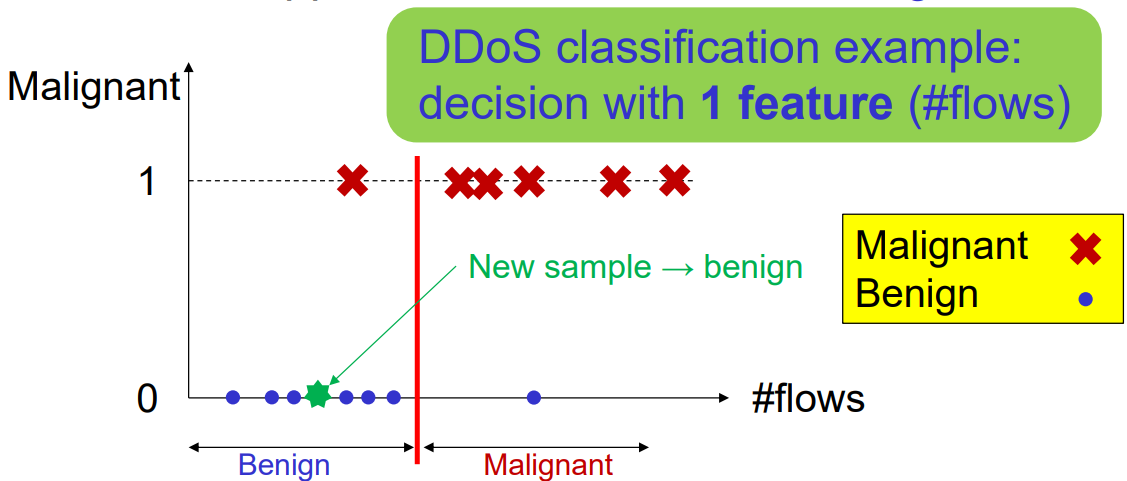
\includegraphics[width=0.6\textwidth]{img/supervised1.png}
\end{figure}

\paragraph{Decisione con 2 feature.}
Lo scenario diventa più realistico introducendo una seconda dimensione.
La figura mostra un piano cartesiano bidimensionale dove l'asse delle
ascisse rappresenta il numero di flussi (\texttt{\#flows}) e l'asse
delle ordinate rappresenta la dimensione dei pacchetti
(\textit{Size}). I dati di addestramento sono sparsi sul piano: i punti
\textit{``Benign''} si concentrano in una zona specifica (basso numero
di flussi, dimensione variabile), mentre i punti
\textit{``Malignant''} occupano un'altra regione. L'algoritmo apprende
una funzione (\textit{learned function}), rappresentata come un confine
di separazione (\textit{Separation Boundary}), che divide il piano in
due aree distinte. Quando viene introdotto un nuovo campione, la sua
posizione nel piano porterà il sistema a classificarlo come maligno se
cade oltre il confine.

\begin{figure}[H]
    \centering
    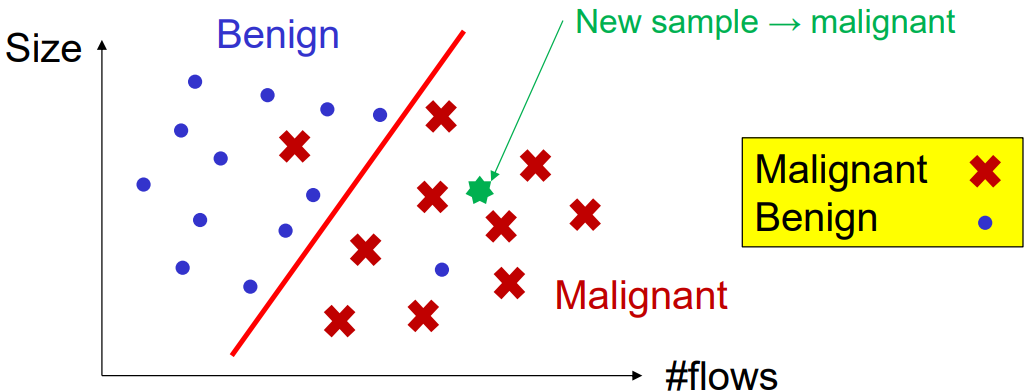
\includegraphics[width=0.6\textwidth]{img/supervised2.png}
\end{figure}

% ............................................................
\subsubsection{Apprendimento non Supervisionato (Unsupervised Learning)}
% ............................................................

A differenza dell'apprendimento supervisionato, l'apprendimento non
supervisionato opera in condizioni di incertezza maggiore. Al sistema
vengono forniti esclusivamente gli input come dati di addestramento,
senza alcuna etichetta o \textit{``risposta corretta''}. Il compito
dell'algoritmo non è predire un valore noto, ma esplorare i dati per
trovare strutture intrinseche nel \textit{``mondo''} osservato.

Gli obiettivi principali in questo paradigma includono:

\begin{itemize}
    \item \textbf{Scoprire Cluster}: identificare raggruppamenti naturali di dati simili.
    \item \textbf{Scoprire Manifold}: trovare superfici o strutture
    geometriche di dimensione inferiore su cui i dati risiedono.
    \item \textbf{Caratterizzare le aree dello spazio}: definire la
    probabilistica delle regioni in cui si distribuiscono i dati.
\end{itemize}

\paragraph{Density Estimation}
Una distribuzione di punti sull'asse $X$ viene approssimata da una
funzione $f(x)$ che modella la densità di probabilità per ogni area
dello spazio. Graficamente, la curva si alza in corrispondenza delle
concentrazioni di punti e si abbassa dove i dati sono scarsi,
permettendo di modellare la probabilità che un dato evento si verifichi.

\paragraph{Clustering}
La figura mostra un piano cartesiano con due assi (\textit{Feature A} e
\textit{Feature B}). I dati sono visibilmente separati in due gruppi
distinti. L'algoritmo, pur non sapendo cosa rappresentino quei punti, è
in grado di circondare questi gruppi (\textit{cluster}) identificando
che essi rappresentano comportamenti simili senza avere modelli
predefiniti.

\paragraph{Embedding}
I punti disposti lungo una forma curva a \textit{``ferro di cavallo''}
nel piano vengono modellati da una linea che ne segue la distribuzione.
Questo rappresenta il concetto di scoprire un \textit{manifold} a bassa
dimensione (una linea unidimensionale) vicino alla quale vivono i dati,
permettendo di semplificare la complessità dimensionale del dataset
originale.

\begin{figure}[H]
    \centering
    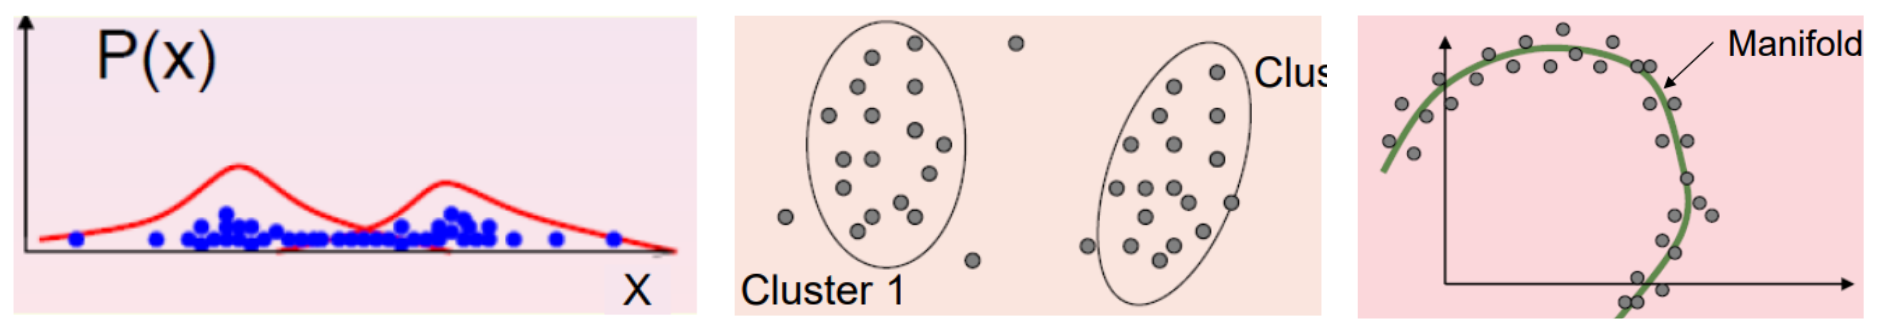
\includegraphics[width=0.9\textwidth]{img/unsupervised.png}
\end{figure}

% ------------------------------------------------------------
\subsubsection{La Sfida dell'Apprendimento (Learning Theory)}
% ------------------------------------------------------------

Il nucleo tecnico del Machine Learning risiede nella capacità di
generalizzazione. Si sottolinea una difficoltà fondamentale intrinseca a
qualsiasi processo di apprendimento induttivo: la discrepanza tra la
finitezza dei dati osservati e l'infinità del dominio di applicazione.

% ............................................................
\paragraph{Derivare Relazioni per Domini Infiniti}
% ............................................................

Il problema centrale è così formulato: dato un ammontare finito di dati
di addestramento, il sistema deve derivare una relazione (o funzione)
valida per un dominio infinito. In termini matematici e logici, esiste
un numero infinito di possibili relazioni che possono spiegare o passare
attraverso un set finito di punti.

\begin{figure}[H]
    \centering
    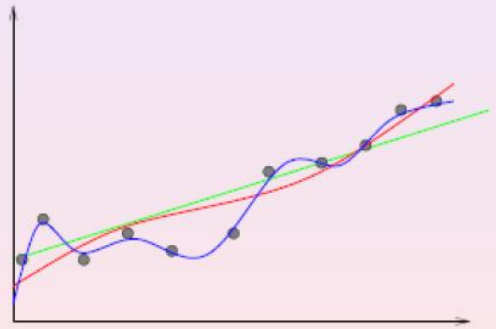
\includegraphics[width=0.5\textwidth]{img/learning.png}
\end{figure}

La figura illustrativa mostra un grafico cartesiano con una serie di
punti neri (i dati di addestramento) disposti con andamento
generalmente crescente ma irregolare. Vengono tracciate tre diverse
curve (funzioni) che tentano di interpretare questi dati:

\begin{enumerate}
    \item \textbf{Una linea retta (verde)}: approssima l'andamento generale 
    ma ignora le variazioni locali dei punti.
    \item \textbf{Una curva sinusoidale complessa (blu)}: passa
    esattamente attraverso ogni singolo punto, seguendo ogni
    oscillazione.
    \item \textbf{Una curva morbida intermedia (rossa)}: segue il trend ma 
    non tocca tutti i punti.
\end{enumerate}

% ............................................................
\subsubsection{Il Problema dell'Overfitting e la Selezione della Relazione}
% ............................................................

Questa rappresentazione visiva introduce la domanda chiave:
\textit{``Which relation is more appropriate?''} (Quale relazione è più
appropriata?).

\begin{itemize}
    \item \textbf{La curva blu}, pur avendo errore zero sui dati di
    training, è probabilmente vittima di \textit{overfitting}: ha
    \textit{``memorizzato''} il rumore dei dati finiti invece di
    apprendere la legge generale del dominio infinito. È troppo
    complessa.
    \item \textbf{La linea verde} potrebbe essere troppo semplice
    (\textit{underfitting}), non catturando la vera natura del
    fenomeno.
\end{itemize}

La sfida dell'apprendimento, quindi, non è solo trovare una funzione che
si adatti ai dati passati, ma selezionare quella che meglio approssima
la verità del dominio infinito sottostante, bilanciando complessità e
accuratezza. Questo concetto si ricollega direttamente al principio del
\textbf{Rasoio di Occam}, che suggerisce di preferire l'ipotesi più
semplice che si adatta ai dati.
